	\section{Dispositif d'assistance (UO 2.3.1 à 2.3.3)}
	\subsection{Compréhension du besoin et démarche proposée}
	\subsubsection{Enjeux}
	Un des enjeux majeurs du lot 2 est de mettre en place un dispositif d’assistance. Ce dernier doit assurer un service d’assistance permanent pour le MOA. Ce service devra être disponible au plus tard 20 jours ouvrés après la notification du marché.
	
	Il est capital pour le MOA que toutes les demandes et tous les incidents inhérents au marché soient pris en compte par le dispositif d’assistance dans des délais corrects et définis.
	
	Notre collaboration totale et pro active est demandée pour ce projet. Il est demandé un travail appliqué et global. En effet, le périmètre de cette UO ne se limite pas seulement au logiciel mais à l’ensemble des composants de l'environnement d'exécution.
	
	Le dispositif sera ouvert aux collaborateurs du MOA et à des acteurs clairement identifiés au préalable. Un niveau d’habilitation sera assigné à chacune des entités afin d’identifier leurs droits en termes de type d’assistance.
	
	Le dispositif mis en place devra être efficace et réactif, il devra donner l’assurance au MOA de pouvoir régler les problèmes détectés et de répondre aux demandes rapidement et efficacement.
	
	\subsubsection{Méthodologie}
	En cas de problème ou de demande, le dispositif d’assistance sera accessible par téléphone, courriel ou site web dédié. Pauline \bsc{Marechal} sera responsable de traiter la demande et d’organiser une réponse adéquate au problème. 
	
	\begin{figure}
	\centering
	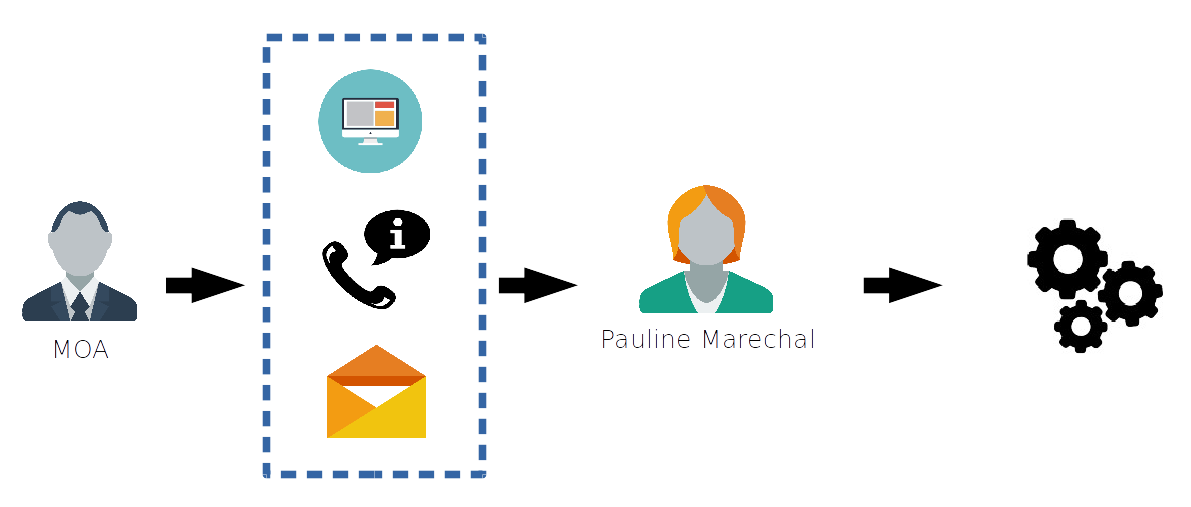
\includegraphics[width=0.8\linewidth]{images/chap3/assistance}
	\caption{Méthodologie d'assistance}
	\label{fig:assistance}
	\end{figure}
	
La réponse devra alors suivre les procédures prédéfinies en fonction du contexte de la demande :
\begin{description}
	\item[En cas d'incident] Une qualification systématique de l’incident devra être donnée. Un diagnostic devra alors être fait et permettra de décrire les comportements des logiciels et systèmes impliqués.~\\
	Le comportement défectueux devra alors être corrigé. Une maintenance évolutive peut également être nécessaire dans le cas de changement de contexte (logiciel ou des infrastructures).
	\item[En cas de demande d'information] La personne responsable du dispositif d’assistance répondra aux demandes d’information si elle possède les qualifications concernant ces informations. Sinon, elle devra identifier le membre de l’équipe capable d’informer de façon précise la personne sur le sujet et  la mettra en contact avec celle-ci.
	\item[En cas de demande d'évolution] Pour toute demande d’évolution notre équipe devra étudier la faisabilité de cette évolution, mais également déterminer les personnes les plus habilitées à mettre en place cette évolution de manière efficace.~\\	
	Le système devra être disponible en continu de 8h00 à 18h00, cela dans l’optique de fournir un service utile et efficace au MOA.		
\end{description}
	

	\subsubsection{Points forts}
	Nos équipes disposent d’une certaine expérience dans le domaine ce qui la rend très efficace dans ce genre de situations que ce soit au niveau de la rapidité d’exécution des demandes, mais également sur la qualité du traitement de celles-ci.
	
	\subsection{Compétences de l'équipe dédiée spécifiquement à l'UO}	
	Pauline Marechal sera responsable de cette UO. Elle possède de réelles compétences en terme de communication et possède un esprit de synthèse parfaitement adapté à cette tâche.
	
	Au cours de sa carrière, elle a eu l’occasion de prendre à sa charge des projets comme la mise en place d’un service d’assistance pour les employés d’Air France.
	
	\subsection{Moyens techniques}
	Nous allons mettre en place un système d'assistance complet et efficace pour le MOA. Celui-ci devra être composé des éléments suivants:
	
	Des téléphones pour les membres de l’équipe.
	Des boites mails.
	Une plateforme internet pour rapporter les bogues.
	
	De plus, Pauline devra utiliser les issues GitHub pour affecter les tâches de corrections ou les demandes d’évolutions et d’informations.